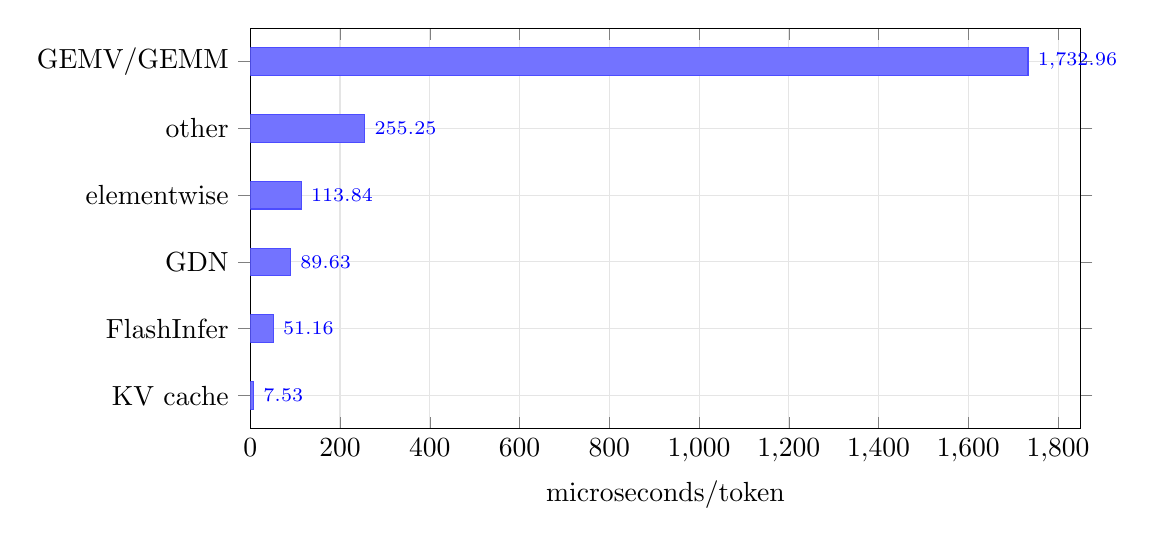
\begin{tikzpicture}
\begin{axis}[
    xbar,
    width=\linewidth,
    height=0.55\linewidth,
    xmin=0,
    xmax=1850,
    xlabel={microseconds/token},
    symbolic y coords={KV cache,FlashInfer,GDN,elementwise,other,GEMV/GEMM},
    ytick=data,
    nodes near coords,
    nodes near coords align={horizontal},
    every node near coord/.append style={font=\scriptsize},
    grid=major,
    major grid style={draw=black!10},
]
\addplot+[fill=blue!55, draw=blue!70] coordinates {
    (7.533,KV cache)
    (51.158,FlashInfer)
    (89.634,GDN)
    (113.838,elementwise)
    (255.254,other)
    (1732.960,GEMV/GEMM)
};
\end{axis}
\end{tikzpicture}
